% Q2 NER section

\subsection{Problem Formulation}
Named Entity Recognition (NER) is a sequence labeling task. Given a token sequence $x = (x_1, \dots, x_n)$, the model predicts a BIO tag sequence $y = (y_1, \dots, y_n)$, where each $y_i \in \{\texttt{O}, \texttt{B-}t, \texttt{I-}t\}$ and $t \in \{\texttt{PER}, \texttt{ORG}, \texttt{LOC}, \texttt{MISC}\}$. We evaluate entity-level precision, recall, and F1 using the \texttt{seqeval} metric.

\subsection{Dataset Description}
We use the CoNLL-2003 dataset with official train/validation/test splits. The label inventory contains 9 BIO tags: \texttt{O}, \texttt{B/I-PER}, \texttt{B/I-ORG}, \texttt{B/I-LOC}, \texttt{B/I-MISC}.

\begin{table}[H]
\centering
\caption{CoNLL-2003 dataset statistics.}
\begin{tabular}{lrrrr}
\toprule
\textbf{Split} & \textbf{Sentences} & \textbf{Tokens} & \textbf{Avg Len} & \textbf{Entity \%} \\
\midrule
Train & 14,041 & 203,621 & 14.50 & 16.72 \\
Validation & 3,250 & 51,362 & 15.80 & 16.75 \\
Test & 3,453 & 46,435 & 13.45 & 17.47 \\
\bottomrule
\end{tabular}
\end{table}

\begin{table}[H]
\centering
\caption{Entity token counts per split.}
\begin{tabular}{lrrrr}
\toprule
\textbf{Split} & \textbf{PER} & \textbf{ORG} & \textbf{LOC} & \textbf{MISC} \\
\midrule
Train & 11,128 & 10,025 & 8,297 & 4,593 \\
Validation & 3,149 & 2,092 & 2,094 & 1,268 \\
Test & 2,773 & 2,496 & 1,925 & 918 \\
\bottomrule
\end{tabular}
\end{table}

\subsection{Methodology}
\textbf{BiLSTM-CRF.} We build a word-level vocabulary (20k) and a character vocabulary, initialize word embeddings with GloVe 100d, and use a character BiLSTM to produce subword-aware representations. The final architecture is word+char embeddings $\rightarrow$ BiLSTM $\rightarrow$ linear layer $\rightarrow$ CRF. The CRF models label dependencies and enforces BIO-consistent transitions.

\textbf{BERT token classification.} We use \texttt{bert-base-cased} with a token classification head. Because BERT uses WordPiece tokenization, we align labels by assigning the original label to the first subword and \texttt{-100} to subsequent subwords and special tokens (ignored in the loss). We train for 3 epochs with batch size 16 and learning rate $5\times10^{-5}$.

\subsection{Experimental Setup}
We fix the random seed to 42 and evaluate once on the test split. Early stopping is applied to BiLSTM-CRF based on validation F1 (patience 5). The BERT training time is 138.23 seconds; BiLSTM-CRF timing was logged as 0.0 seconds in the output (likely a timing artifact).

\subsection{Results}
\begin{table}[H]
\centering
\caption{Per-entity and overall results on the test set.}
\begin{tabular}{llccc}
\toprule
\textbf{Entity} & \textbf{Model} & \textbf{Precision} & \textbf{Recall} & \textbf{F1} \\
\midrule
PER & BiLSTM-CRF & 0.9363 & 0.9091 & 0.9225 \\
PER & BERT & 0.9645 & 0.9591 & 0.9618 \\
ORG & BiLSTM-CRF & 0.8712 & 0.8104 & 0.8397 \\
ORG & BERT & 0.8733 & 0.9043 & 0.8885 \\
LOC & BiLSTM-CRF & 0.8972 & 0.9107 & 0.9039 \\
LOC & BERT & 0.9324 & 0.9268 & 0.9296 \\
MISC & BiLSTM-CRF & 0.7356 & 0.7849 & 0.7595 \\
MISC & BERT & 0.7691 & 0.8162 & 0.7920 \\
\midrule
Overall & BiLSTM-CRF & 0.8793 & 0.8651 & 0.8721 \\
Overall & BERT & 0.9024 & 0.9157 & 0.9090 \\
\bottomrule
\end{tabular}
\end{table}

\begin{figure}[H]
\centering
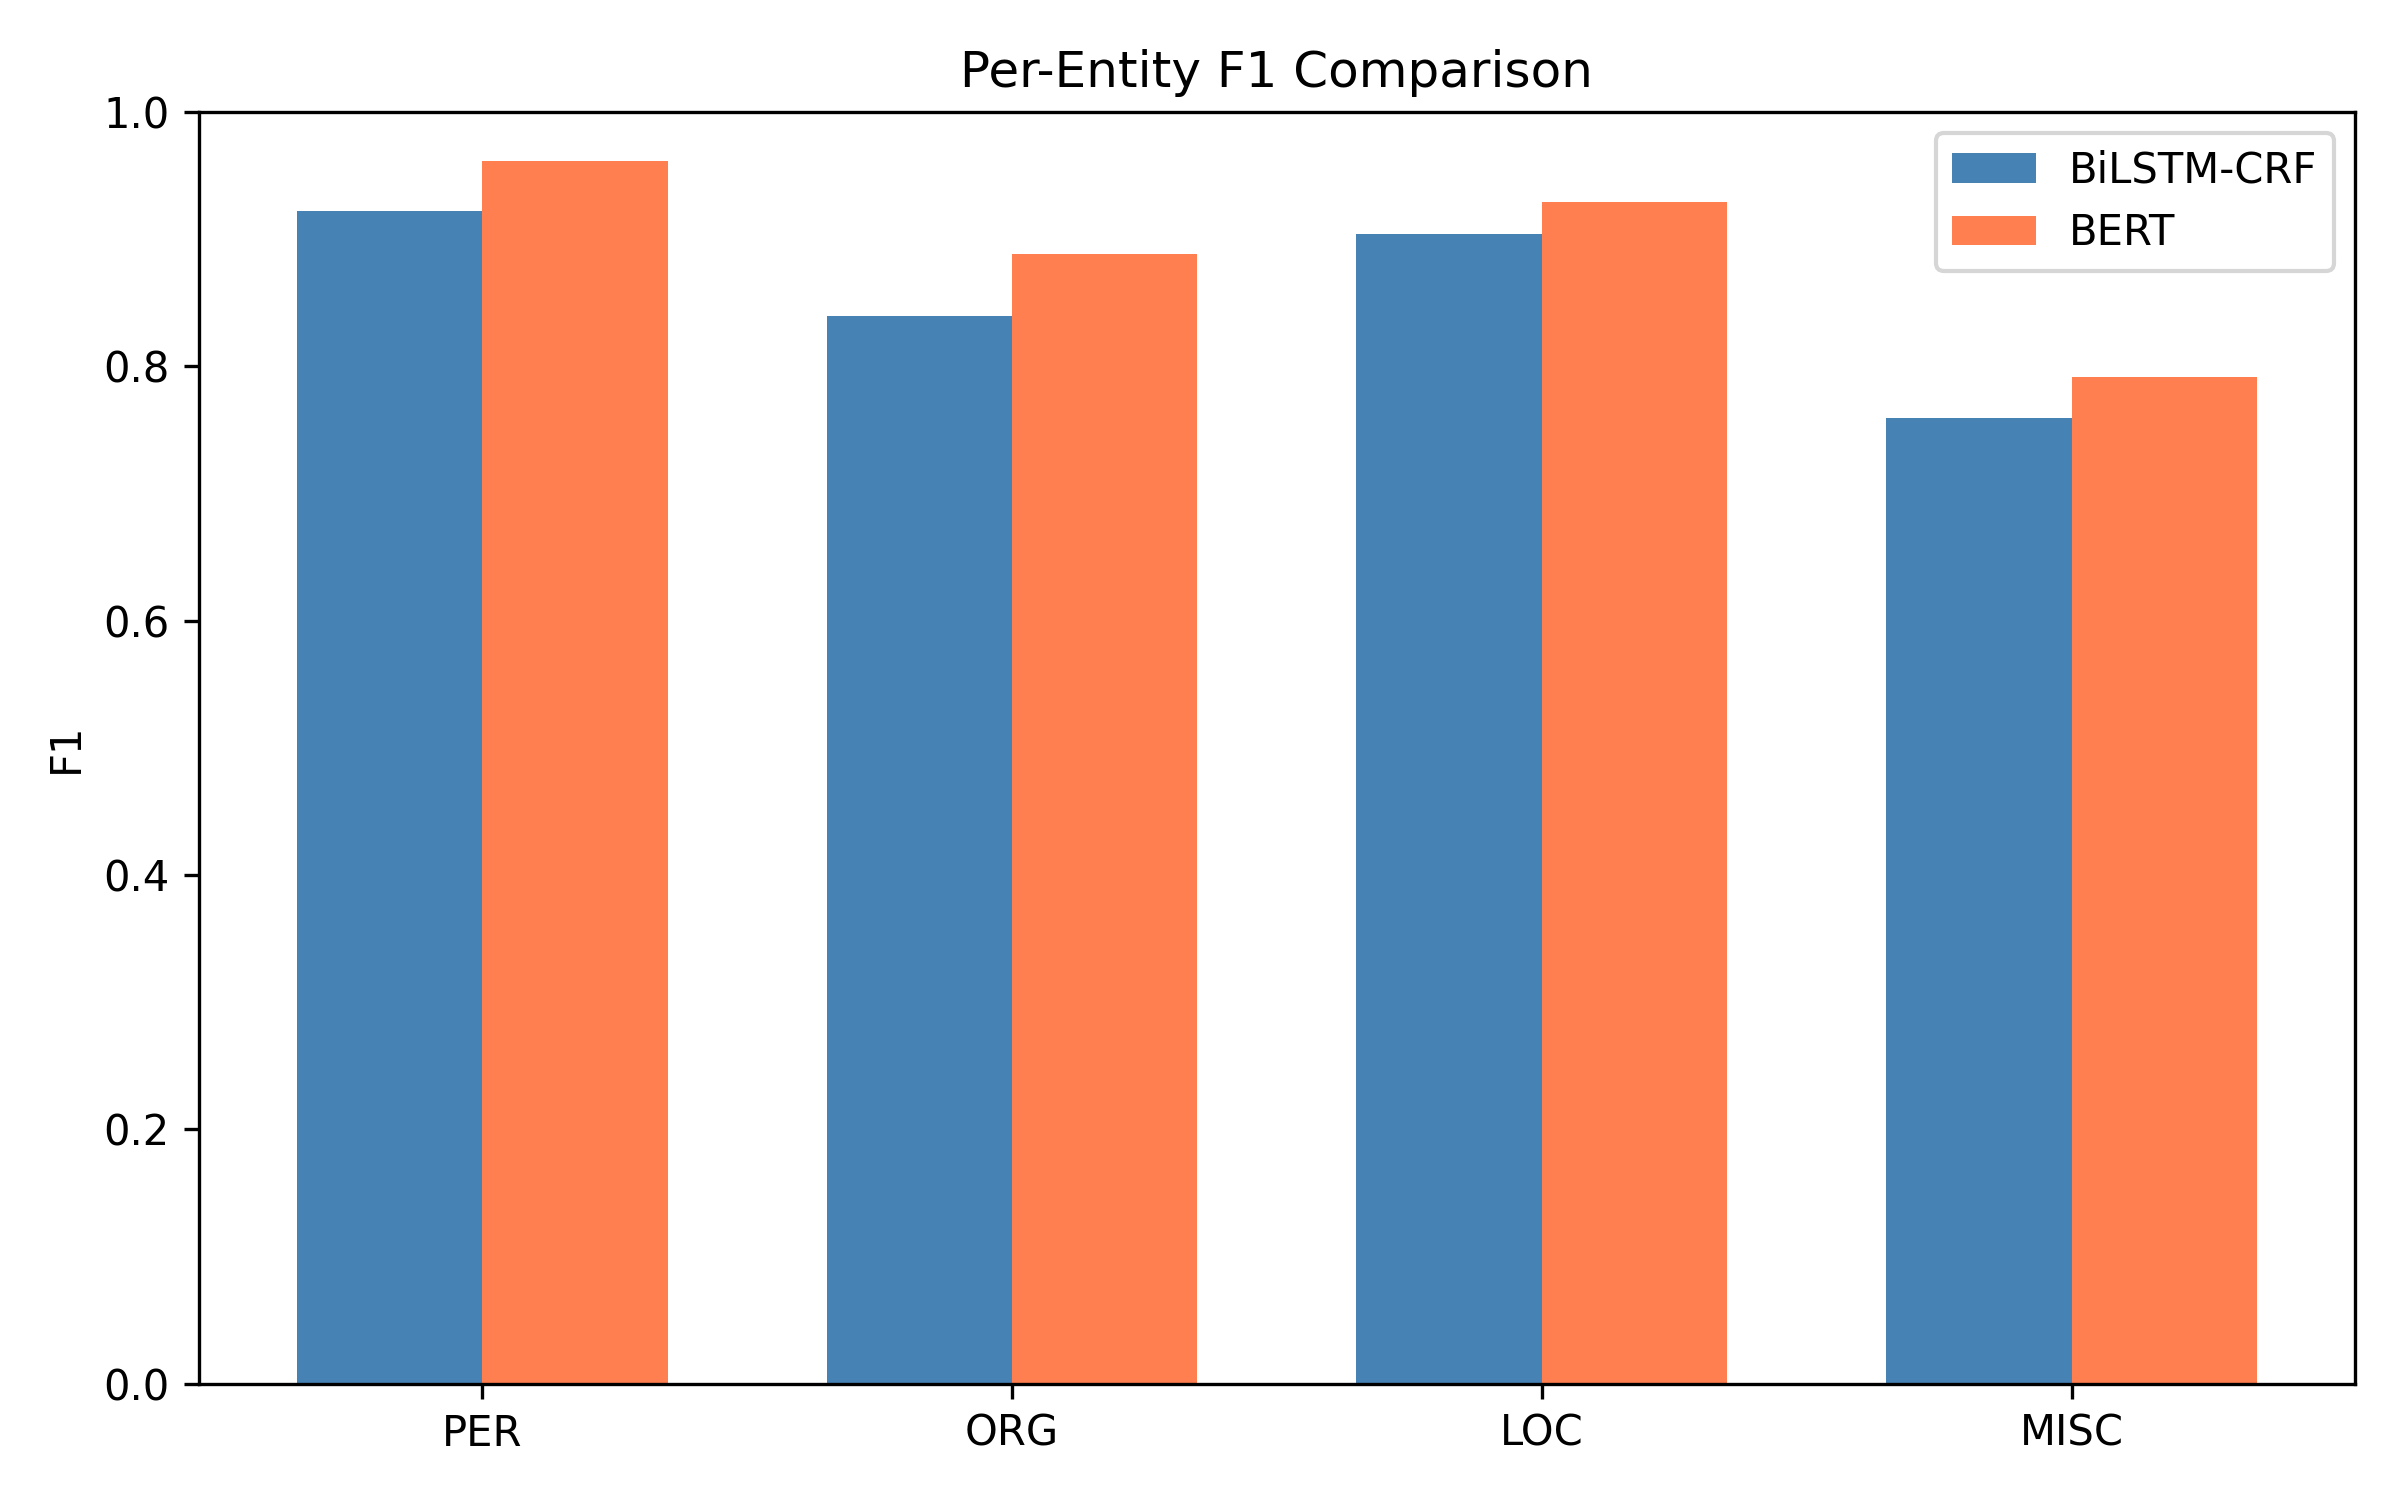
\includegraphics[width=0.75\linewidth]{../q2_ner/outputs/figures/per_entity_f1.png}
\caption{Per-entity F1 comparison between BiLSTM-CRF and BERT.}
\end{figure}

\begin{figure}[H]
\centering
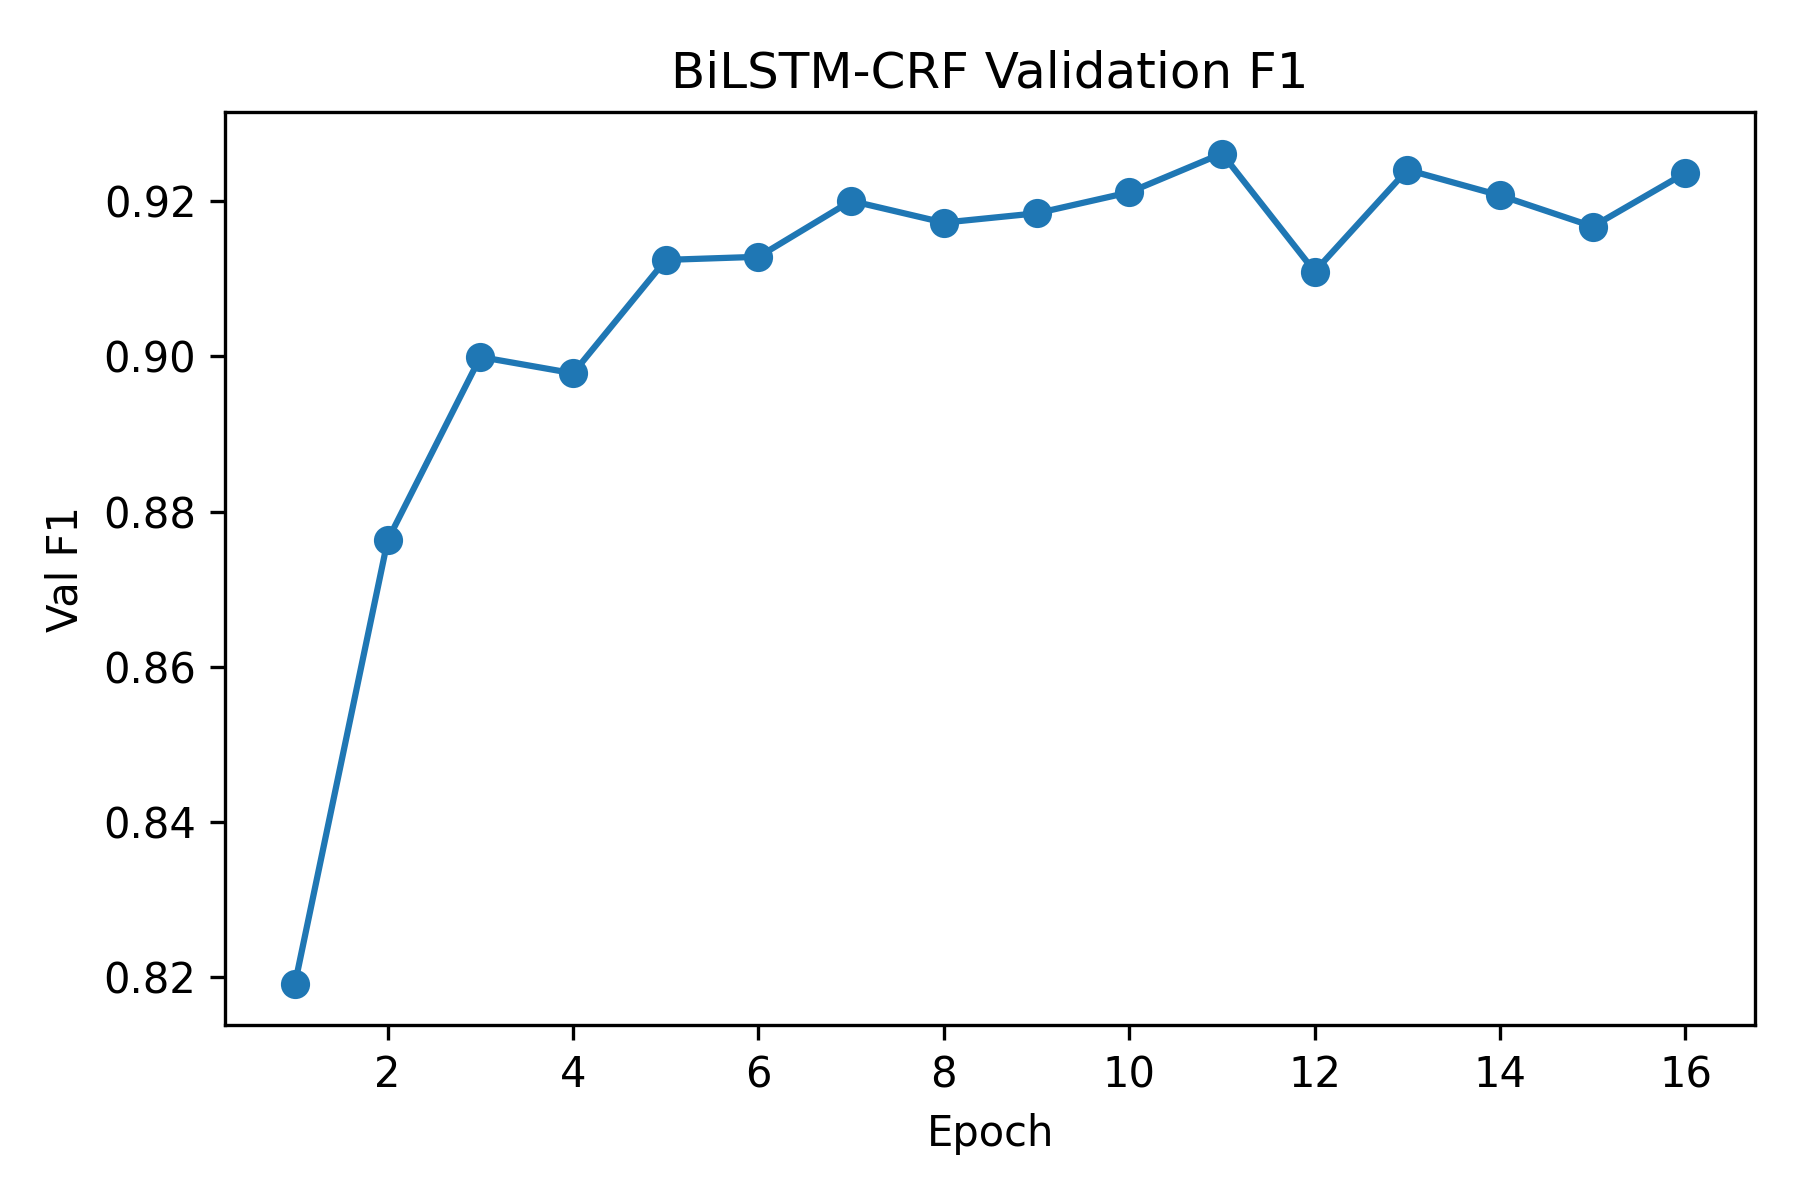
\includegraphics[width=0.65\linewidth]{../q2_ner/outputs/figures/training_bilstm_crf.png}
\caption{BiLSTM-CRF validation F1 across epochs.}
\end{figure}

\begin{figure}[H]
\centering
\begin{subfigure}{0.48\linewidth}
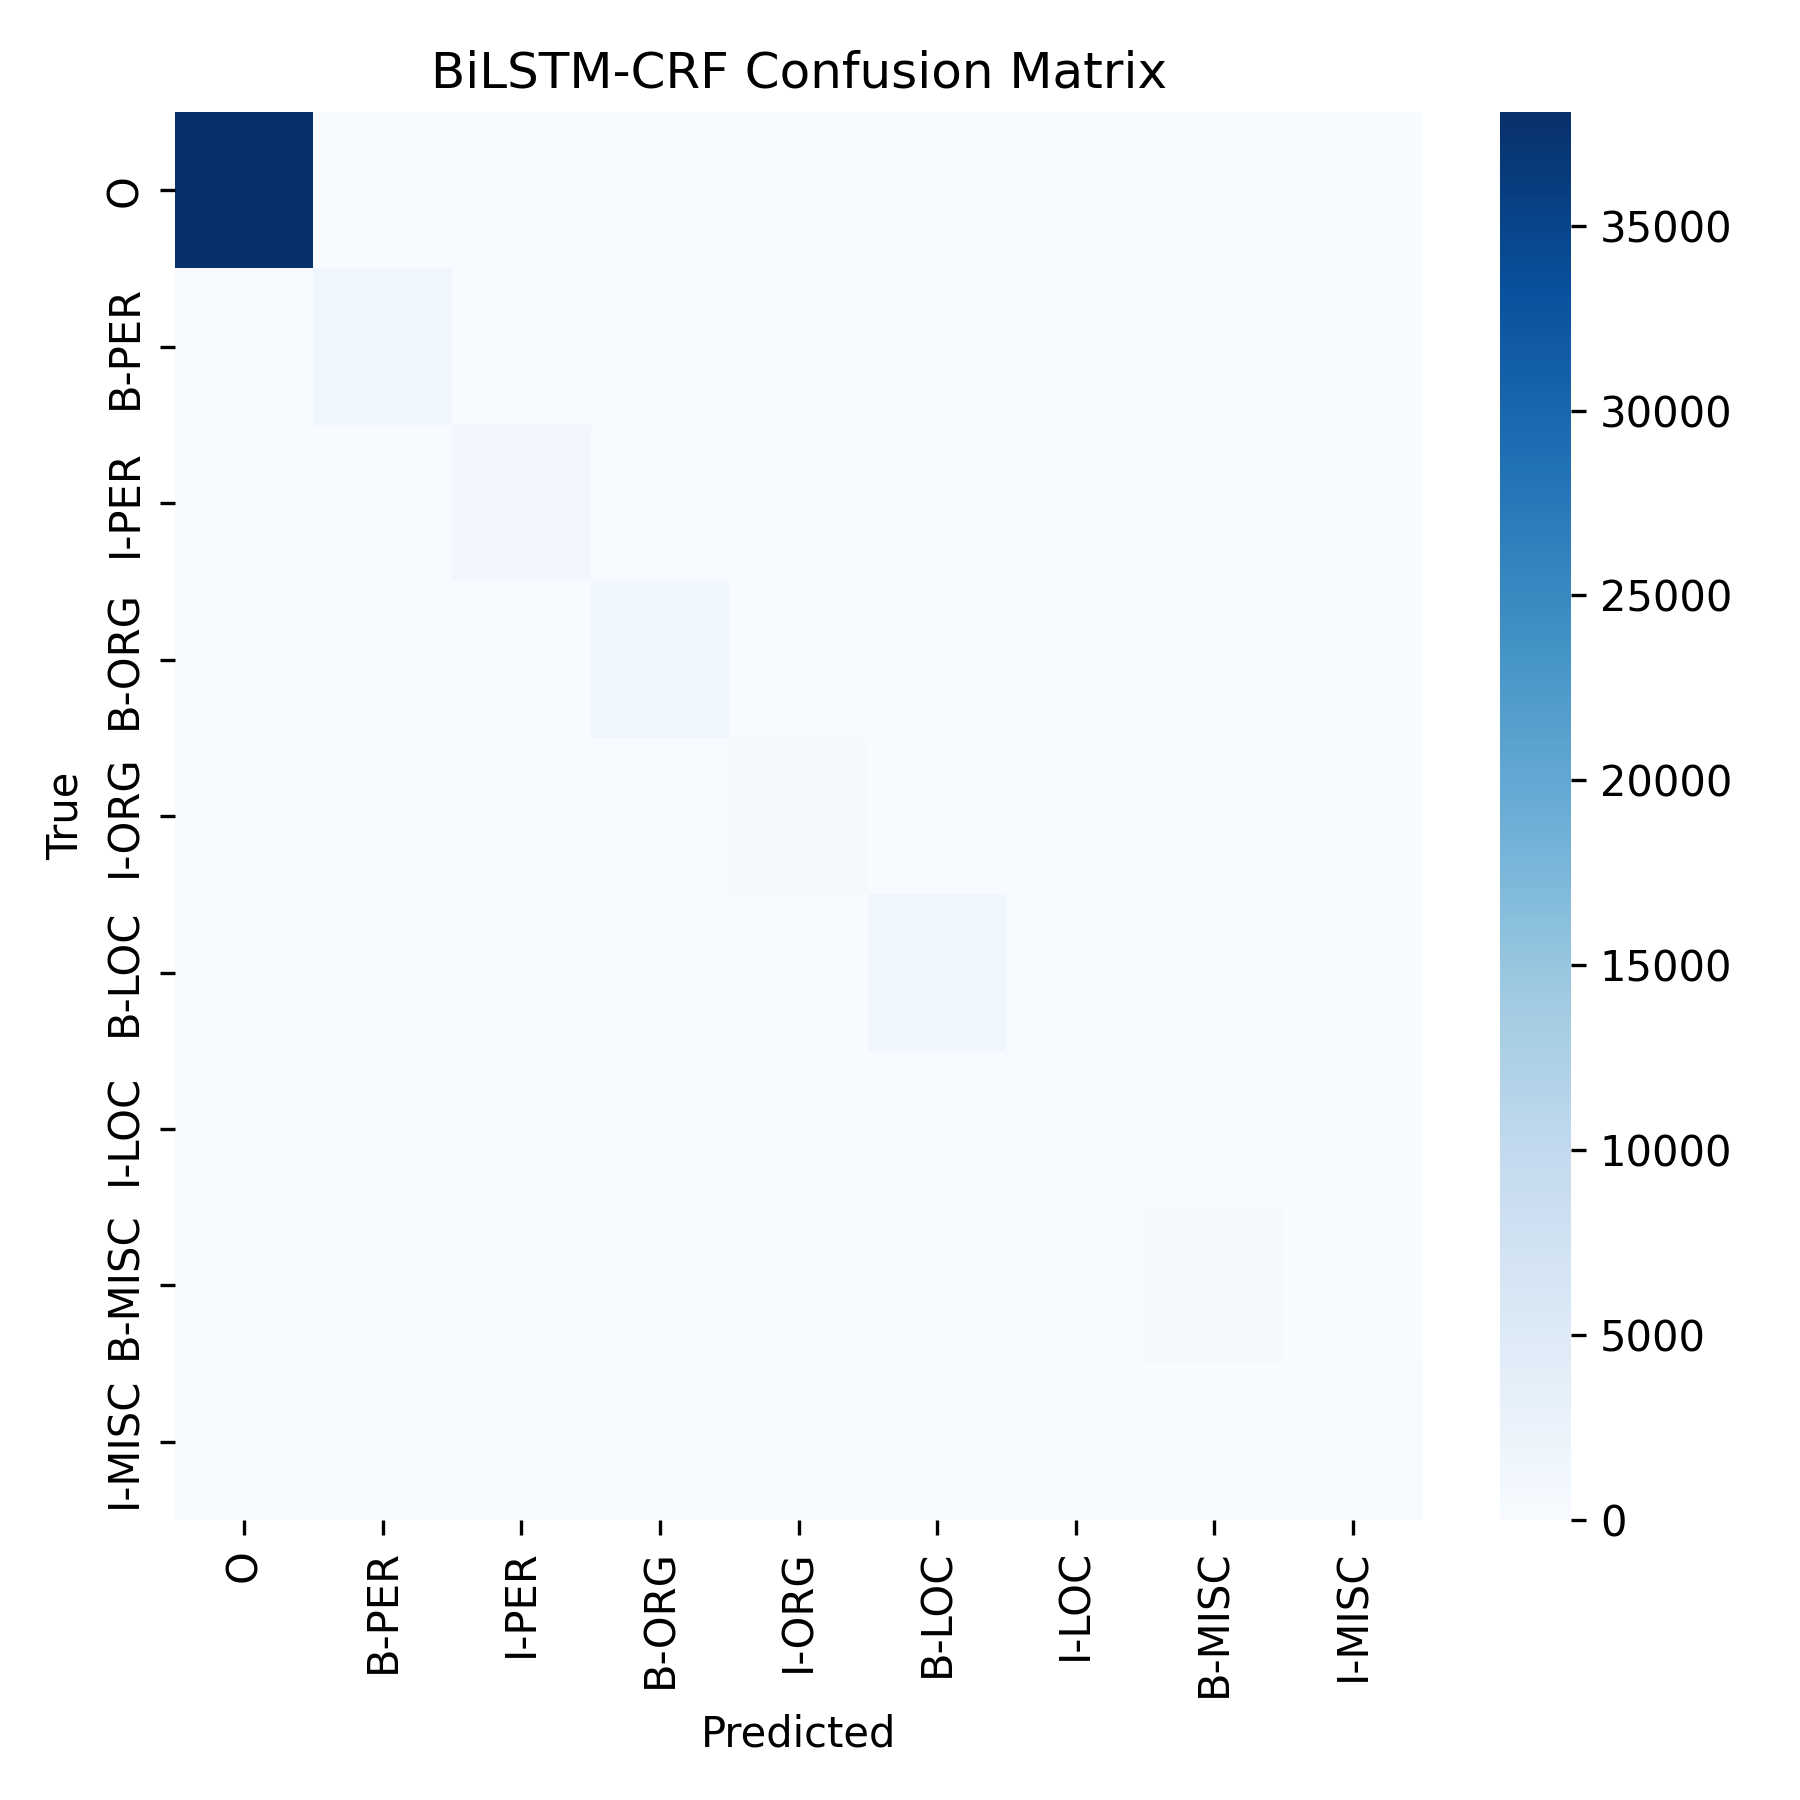
\includegraphics[width=\linewidth]{../q2_ner/outputs/figures/cm_bilstm_crf.png}
\caption{BiLSTM-CRF}
\end{subfigure}
\begin{subfigure}{0.48\linewidth}
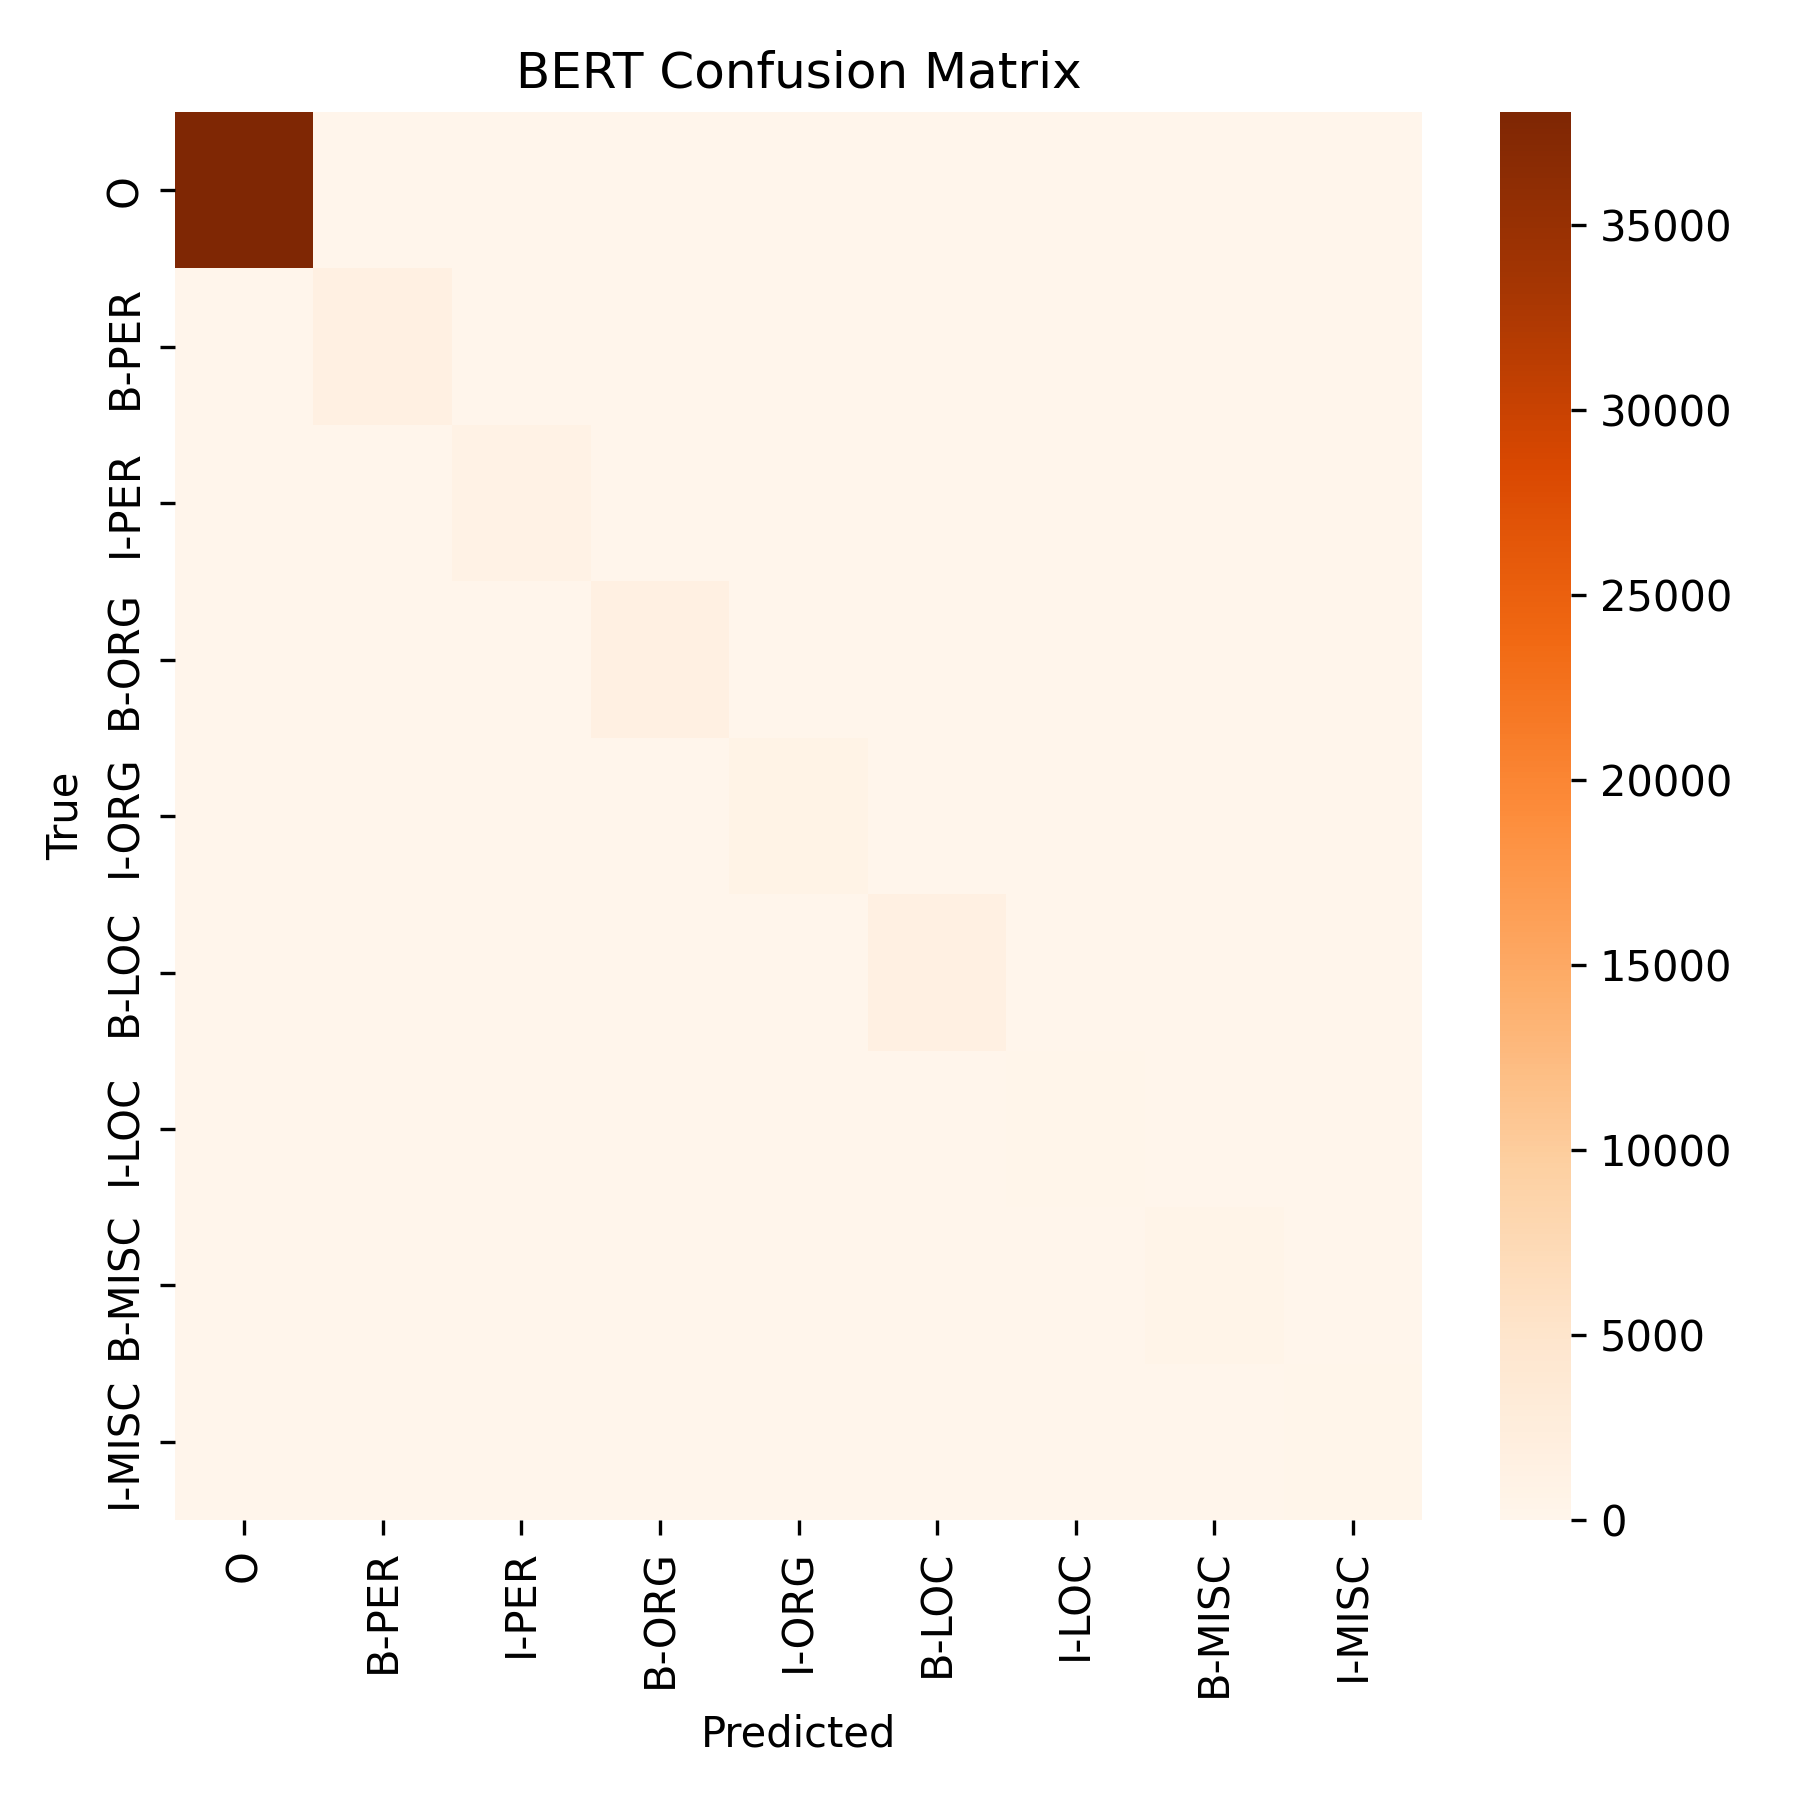
\includegraphics[width=\linewidth]{../q2_ner/outputs/figures/cm_bert.png}
\caption{BERT}
\end{subfigure}
\caption{Confusion matrices over BIO labels.}
\end{figure}

\begin{figure}[H]
\centering
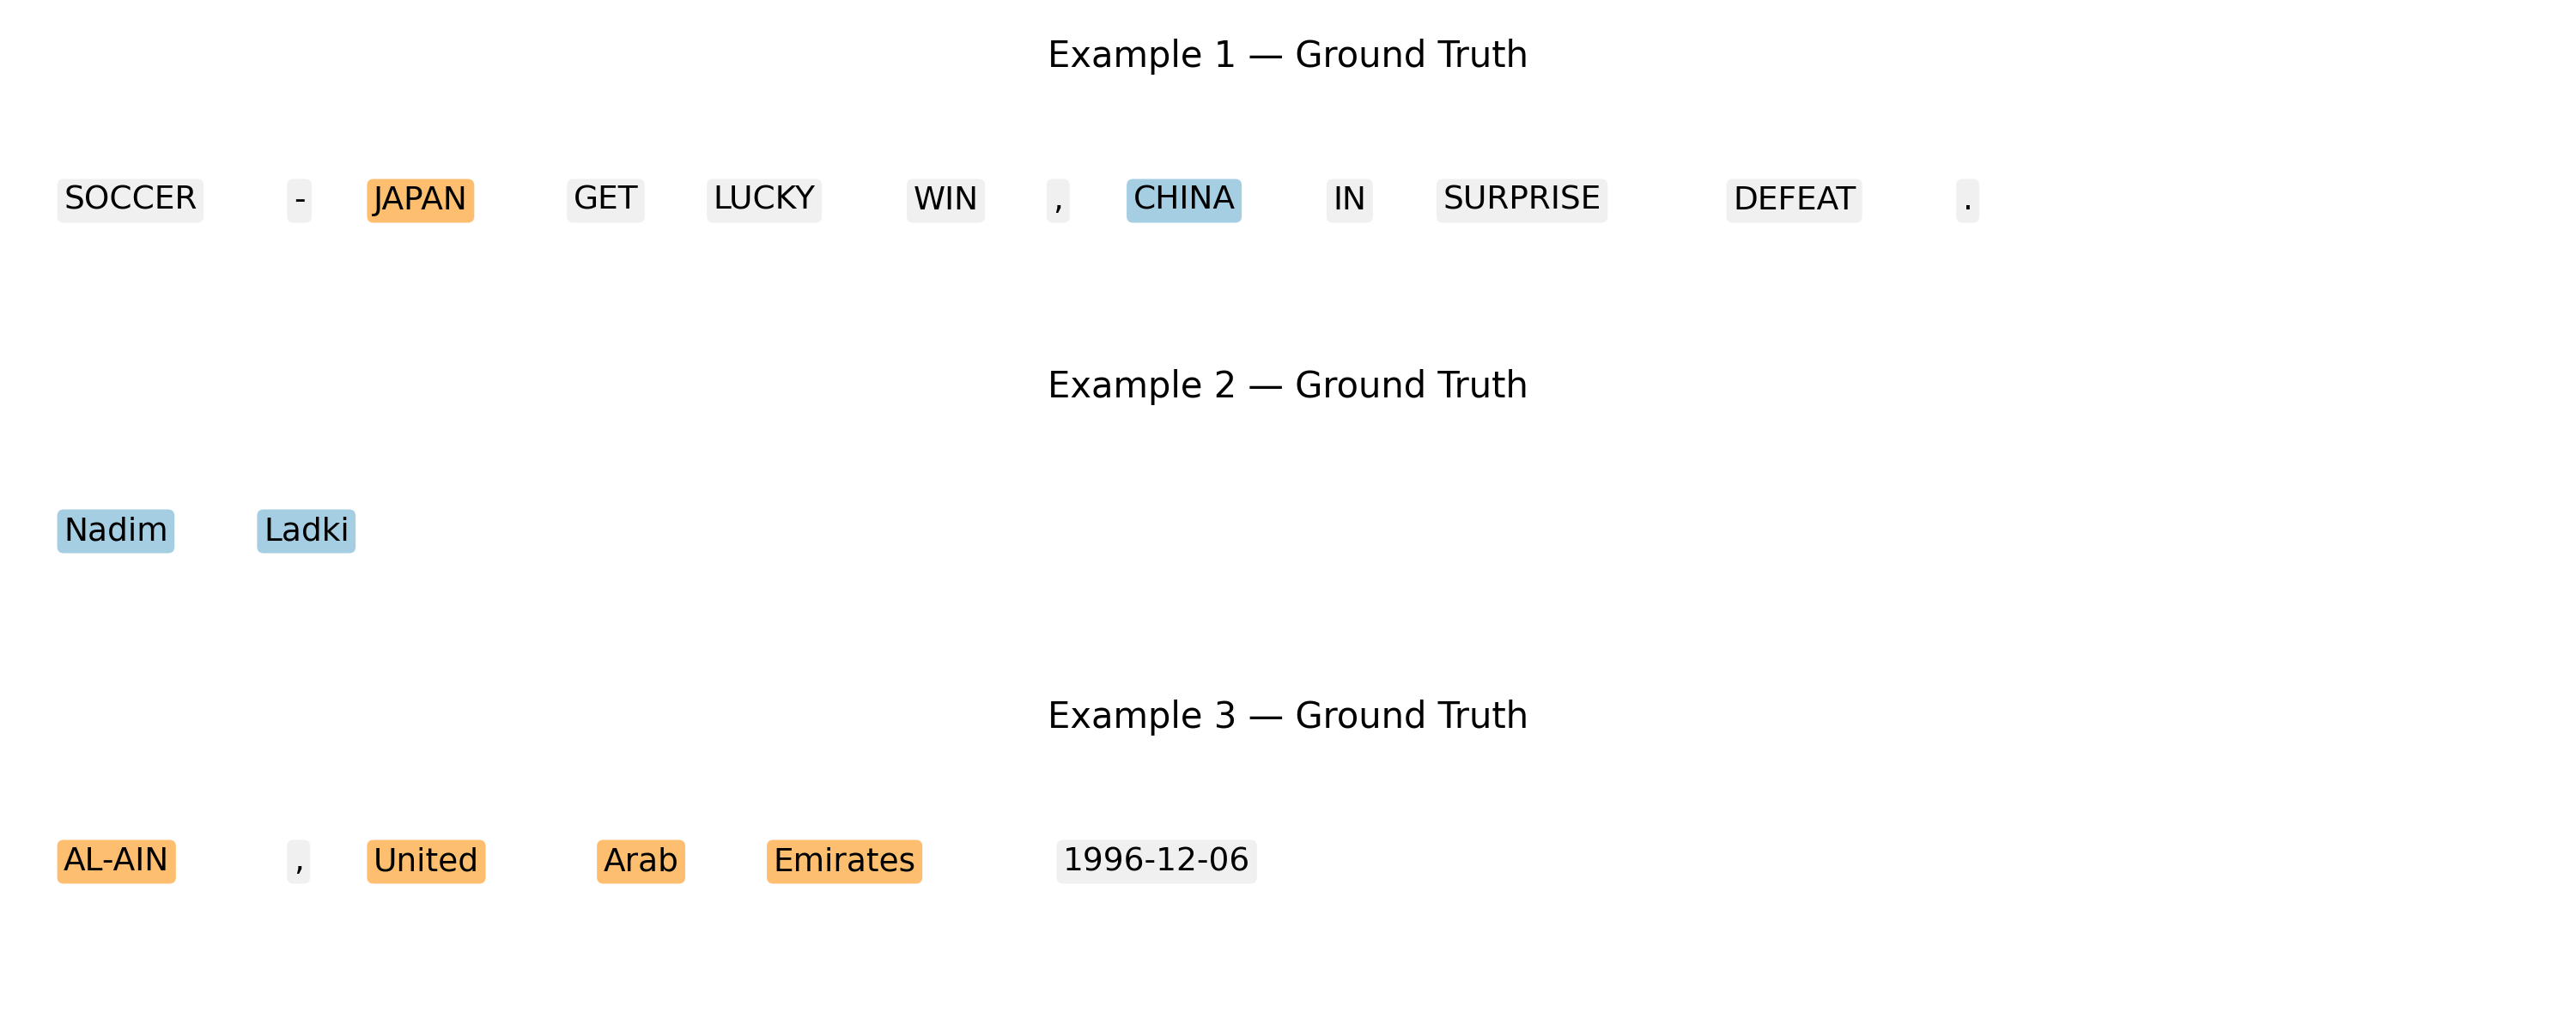
\includegraphics[width=0.90\linewidth]{../q2_ner/outputs/figures/entity_examples.png}
\caption{Example sentences with gold entity labels.}
\end{figure}

\subsection{Error Analysis}
We categorize errors using span-level comparisons on BERT predictions. The counts are: type confusion (317), false positives (139), boundary errors (81), and false negatives (74). Five representative errors are:

\begin{itemize}[leftmargin=*]
\item \textbf{Type confusion (LOC $\rightarrow$ ORG/PER).} Sentence: \texttt{SOCCER - JAPAN GET LUCKY WIN , CHINA IN SURPRISE DEFEAT .} \\ True: \texttt{O O B-LOC O O O O B-PER O O O O} \\ Pred: \texttt{O O B-ORG O O O O B-ORG O O O O}. \\ Hypothesis: country names in sports headlines are often interpreted as organizations.
\item \textbf{False negative (missed PER/LOC).} Sentence: \texttt{RUGBY UNION - CUTTITTA BACK FOR ITALY AFTER A YEAR .} \\ True: \texttt{B-ORG I-ORG O B-PER O O B-LOC O O O O} \\ Pred: \texttt{B-ORG I-ORG O B-ORG O O O O O O O}. \\ Hypothesis: person names in uppercase are confused with organizations, and nearby locations are dropped.
\item \textbf{Boundary error (missing initial token).} Sentence: \texttt{Cuttitta announced his retirement after the 1995 World Cup , ...} \\ True: \texttt{B-PER ... B-MISC I-MISC I-MISC ...} \\ Pred: \texttt{B-PER ... O B-MISC I-MISC ...}. \\ Hypothesis: multi-token event names are truncated.
\item \textbf{Boundary error (invalid BIO start).} Sentence: \texttt{FREESTYLE SKIING-WORLD CUP MOGUL RESULTS .} \\ True: \texttt{O B-MISC I-MISC O O O} \\ Pred: \texttt{O O I-MISC O O O}. \\ Hypothesis: model sometimes emits \texttt{I-} without a preceding \texttt{B-} for hyphenated entities.
\item \textbf{False positive (spurious MISC).} Sentence: \texttt{CRICKET - LARA SUFFERS MORE AUSTRALIAN TOUR MISERY .} \\ True: \texttt{O O B-PER O O O O O O} \\ Pred: \texttt{O O B-MISC O O B-MISC O I-MISC O}. \\ Hypothesis: sports-related phrases are over-labeled as \texttt{MISC}.
\end{itemize}

\subsection{Discussion}
BERT outperforms BiLSTM-CRF overall (0.909 vs 0.872 F1) and across all entity types, with the largest gains on PER and ORG. Both models struggle most with MISC, indicating weaker boundaries for heterogeneous categories. The dominant error type is label confusion, suggesting that headline-style contexts and uppercase tokens blur distinctions between LOC, ORG, and PER. Incorporating gazetteers or additional contextual features could reduce these confusions.
